\documentclass{article}
% Independent first-pass revision; main.tex is preserved.
% Exact-loss tables: docs/reports/v24_optimizer_search_2026-09-10.{pdf,csv,sources.json}
% and docs/reports/v24_mamba_lr_di_10day_2026-09-14.{pdf,csv,sources.json}.
% Figure data and reproducible generator: Graphs/main_v2/README.md.

% if you need to pass options to natbib, use, e.g.:
%     \PassOptionsToPackage{numbers, compress}{natbib}
% before loading neurips_2026

% The authors should use one of these tracks.
% Before accepting by the NeurIPS conference, select one of the options below.
% 0. "default" for submission
\usepackage[preprint]{neurips_2026}
% the "default" option is equal to the "main" option, which is used for the Main Track with double-blind reviewing.
% 1. "main" option is used for the Main Track
%  \usepackage[main]{neurips_2026}
% 2. "position" option is used for the Position Paper Track
%  \usepackage[position]{neurips_2026}
% 3. "eandd" option is used for the Evaluations & Datasets Track
 % \usepackage[eandd]{neurips_2026}
% 4. "creativeai" option is used for the Creative AI Track
%  \usepackage[creativeai]{neurips_2026}
% 5. "sglblindworkshop" option is used for the Workshop with single-blind reviewing
 % \usepackage[sglblindworkshop]{neurips_2026}
% 6. "dblblindworkshop" option is used for the Workshop with double-blind reviewing
%  \usepackage[dblblindworkshop]{neurips_2026}
% 7. "education" option is used for the Education Track
%  \usepackage[education]{neurips_2026}


% After being accepted, the authors should add "final" behind the track to compile a camera-ready version.
% 1. Main Track
 % \usepackage[main, final]{neurips_2026}
% 2. Position Paper Track
%  \usepackage[position, final]{neurips_2026}
% 3. Evaluations & Datasets Track
 % \usepackage[eandd, final]{neurips_2026}
% 4. Creative AI Track
%  \usepackage[creativeai, final]{neurips_2026}
% 5. Workshop with single-blind reviewing
%  \usepackage[sglblindworkshop, final]{neurips_2026}
% 6. Workshop with double-blind reviewing
%  \usepackage[dblblindworkshop, final]{neurips_2026}
% Note. For the workshop paper template, both \title{} and \workshoptitle{} are required, with the former indicating the paper title shown in the title and the latter indicating the workshop title displayed in the footnote.
% For workshops (5., 6.), the authors should add the name of the workshop, "\workshoptitle" command is used to set the workshop title.
% \workshoptitle{WORKSHOP TITLE}
% 7. Education Track
% \usepackage[education, final]{neurips_2026}

% "preprint" option is used for arXiv or other preprint submissions
 % \usepackage[preprint]{neurips_2026}

% to avoid loading the natbib package, add option nonatbib:
%    \usepackage[nonatbib]{neurips_2026}

\usepackage[utf8]{inputenc} % allow utf-8 input
\usepackage[T1]{fontenc}    % use 8-bit T1 fonts
\usepackage{hyperref}       % hyperlinks
\usepackage{url}            % simple URL typesetting
\usepackage{booktabs}       % professional-quality tables
\usepackage{amsfonts}       % blackboard math symbols
\usepackage{nicefrac}       % compact symbols for 1/2, etc.
\usepackage{microtype}      % microtypography
\usepackage{xcolor} 
% colors
\usepackage{amsmath,amssymb,amsthm,mathrsfs,mathtools,amsfonts,physics,bm,bbm,booktabs, gensymb}
\usepackage{graphicx}
\usepackage{subcaption}
\usepackage{placeins}

% Note. For the workshop paper template, both \title{} and \workshoptitle{} are required, with the former indicating the paper title shown in the title and the latter indicating the workshop title displayed in the footnote. 
\title{Capturing non-Markovian effects in weather prediction models}


% The \author macro works with any number of authors. There are two commands
% used to separate the names and addresses of multiple authors: \And and \AND.
%
% Using \And between authors leaves it to LaTeX to determine where to break the
% lines. Using \AND forces a line break at that point. So, if LaTeX puts 3 of 4
% authors names on the first line, and the last on the second line, try using
% \AND instead of \And before the third author name.


\author{
}


\begin{document}


\maketitle


\begin{abstract}
Many existing weather forecasting models are Markovian in their chosen state representation, yet unresolved atmospheric processes can make coarse-grained dynamics history dependent. We introduce GraphCast–Mamba, which augments a frozen, pretrained \(1^\circ\) GraphCast model with a correction branch combining graph message passing and persistent temporal memory. On a development set of 32 matched forecast starts, selected configurations reduce the original GraphCast loss by approximately 16 over a ten-day rollout and 23 at day ten. These results highlight the potential of learned non-Markovian corrections for improving long-range weather forecasts.
\end{abstract}



\section{Introduction to the architecture}
Turbulent flows are known as a notoriously difficult framework for numerical simulations. One of the common method in such simulations is the \textit{direct numerical simulations} (DNS) that discretize the Navier-Stokes equation to a space and time grid and then simulate directly. Such discretizations, however require a very fine grid resolution scaling as $N_{\textrm{grid}} \sim \left(Re\right)^{\alpha}$ with $\alpha \sim 2.05 $ \cite{yang2021grid}. Insufficient small-scale resolution may leave mean dissipation and enstrophy approximately converged while substantially underestimating high-order moments of velocity gradients, dissipation, and enstrophy, as well as the tails of velocity-gradient distributions and statistics involving second velocity derivatives \cite{DonzisResolutionEffects}.
 While this becomes expensive, a variety of models that regularize the equations on a larger scale, introducing proper dissipative terms at the cost of short time accuracy \cite{Wilson1996Review}. Another approach consists in keeping coarse-grained scales, without non-controlled dissipative approximation, but at a cost of keeping the non-Markovian memory terms \cite{YenTingLinMZ2021,de2026data}.

In this article, we explore the potential of such methods for a weather prediction models.

% Start figure-led discussions with the figure at the top of the same page.
\clearpage
\begin{figure}[!t]
    \centering
    \begin{subfigure}{0.9\linewidth}
        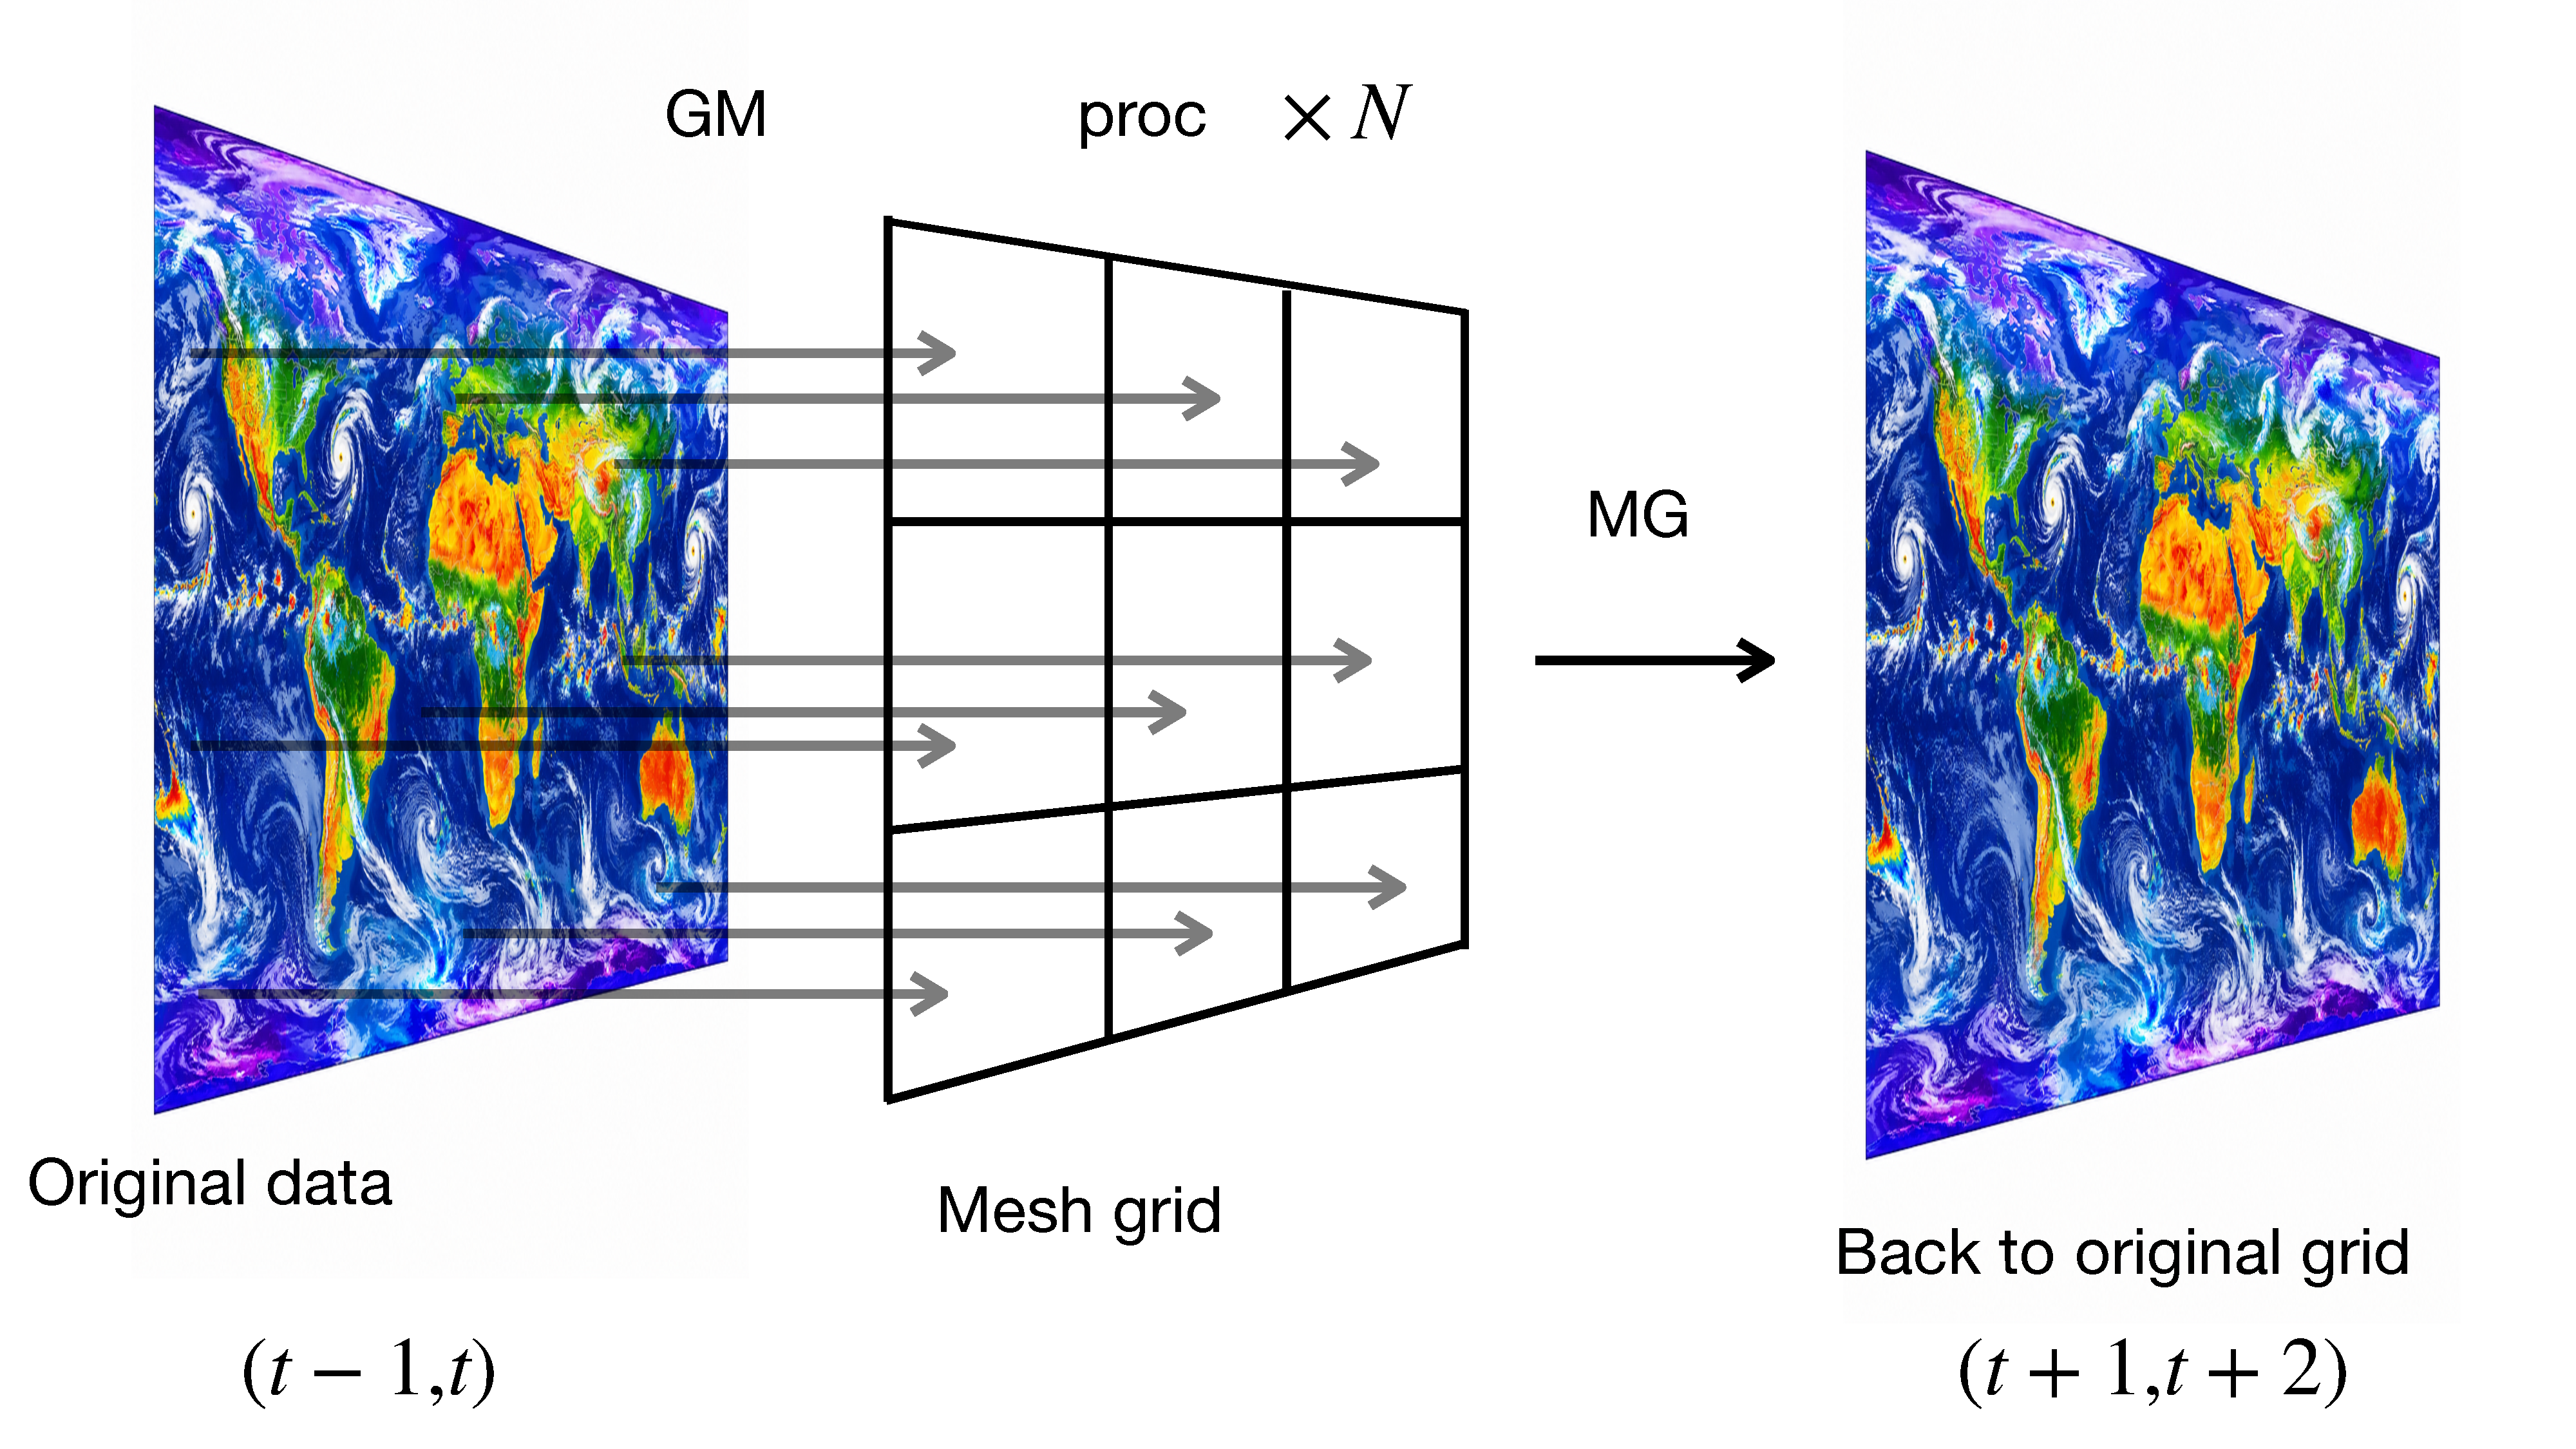
\includegraphics[width=\linewidth]{Pics/GC.pdf}
        \caption{GraphCast maps the input grid to a mesh, performs message passing, and decodes back to the grid.}
    \end{subfigure}
    \begin{subfigure}{0.9\linewidth}
        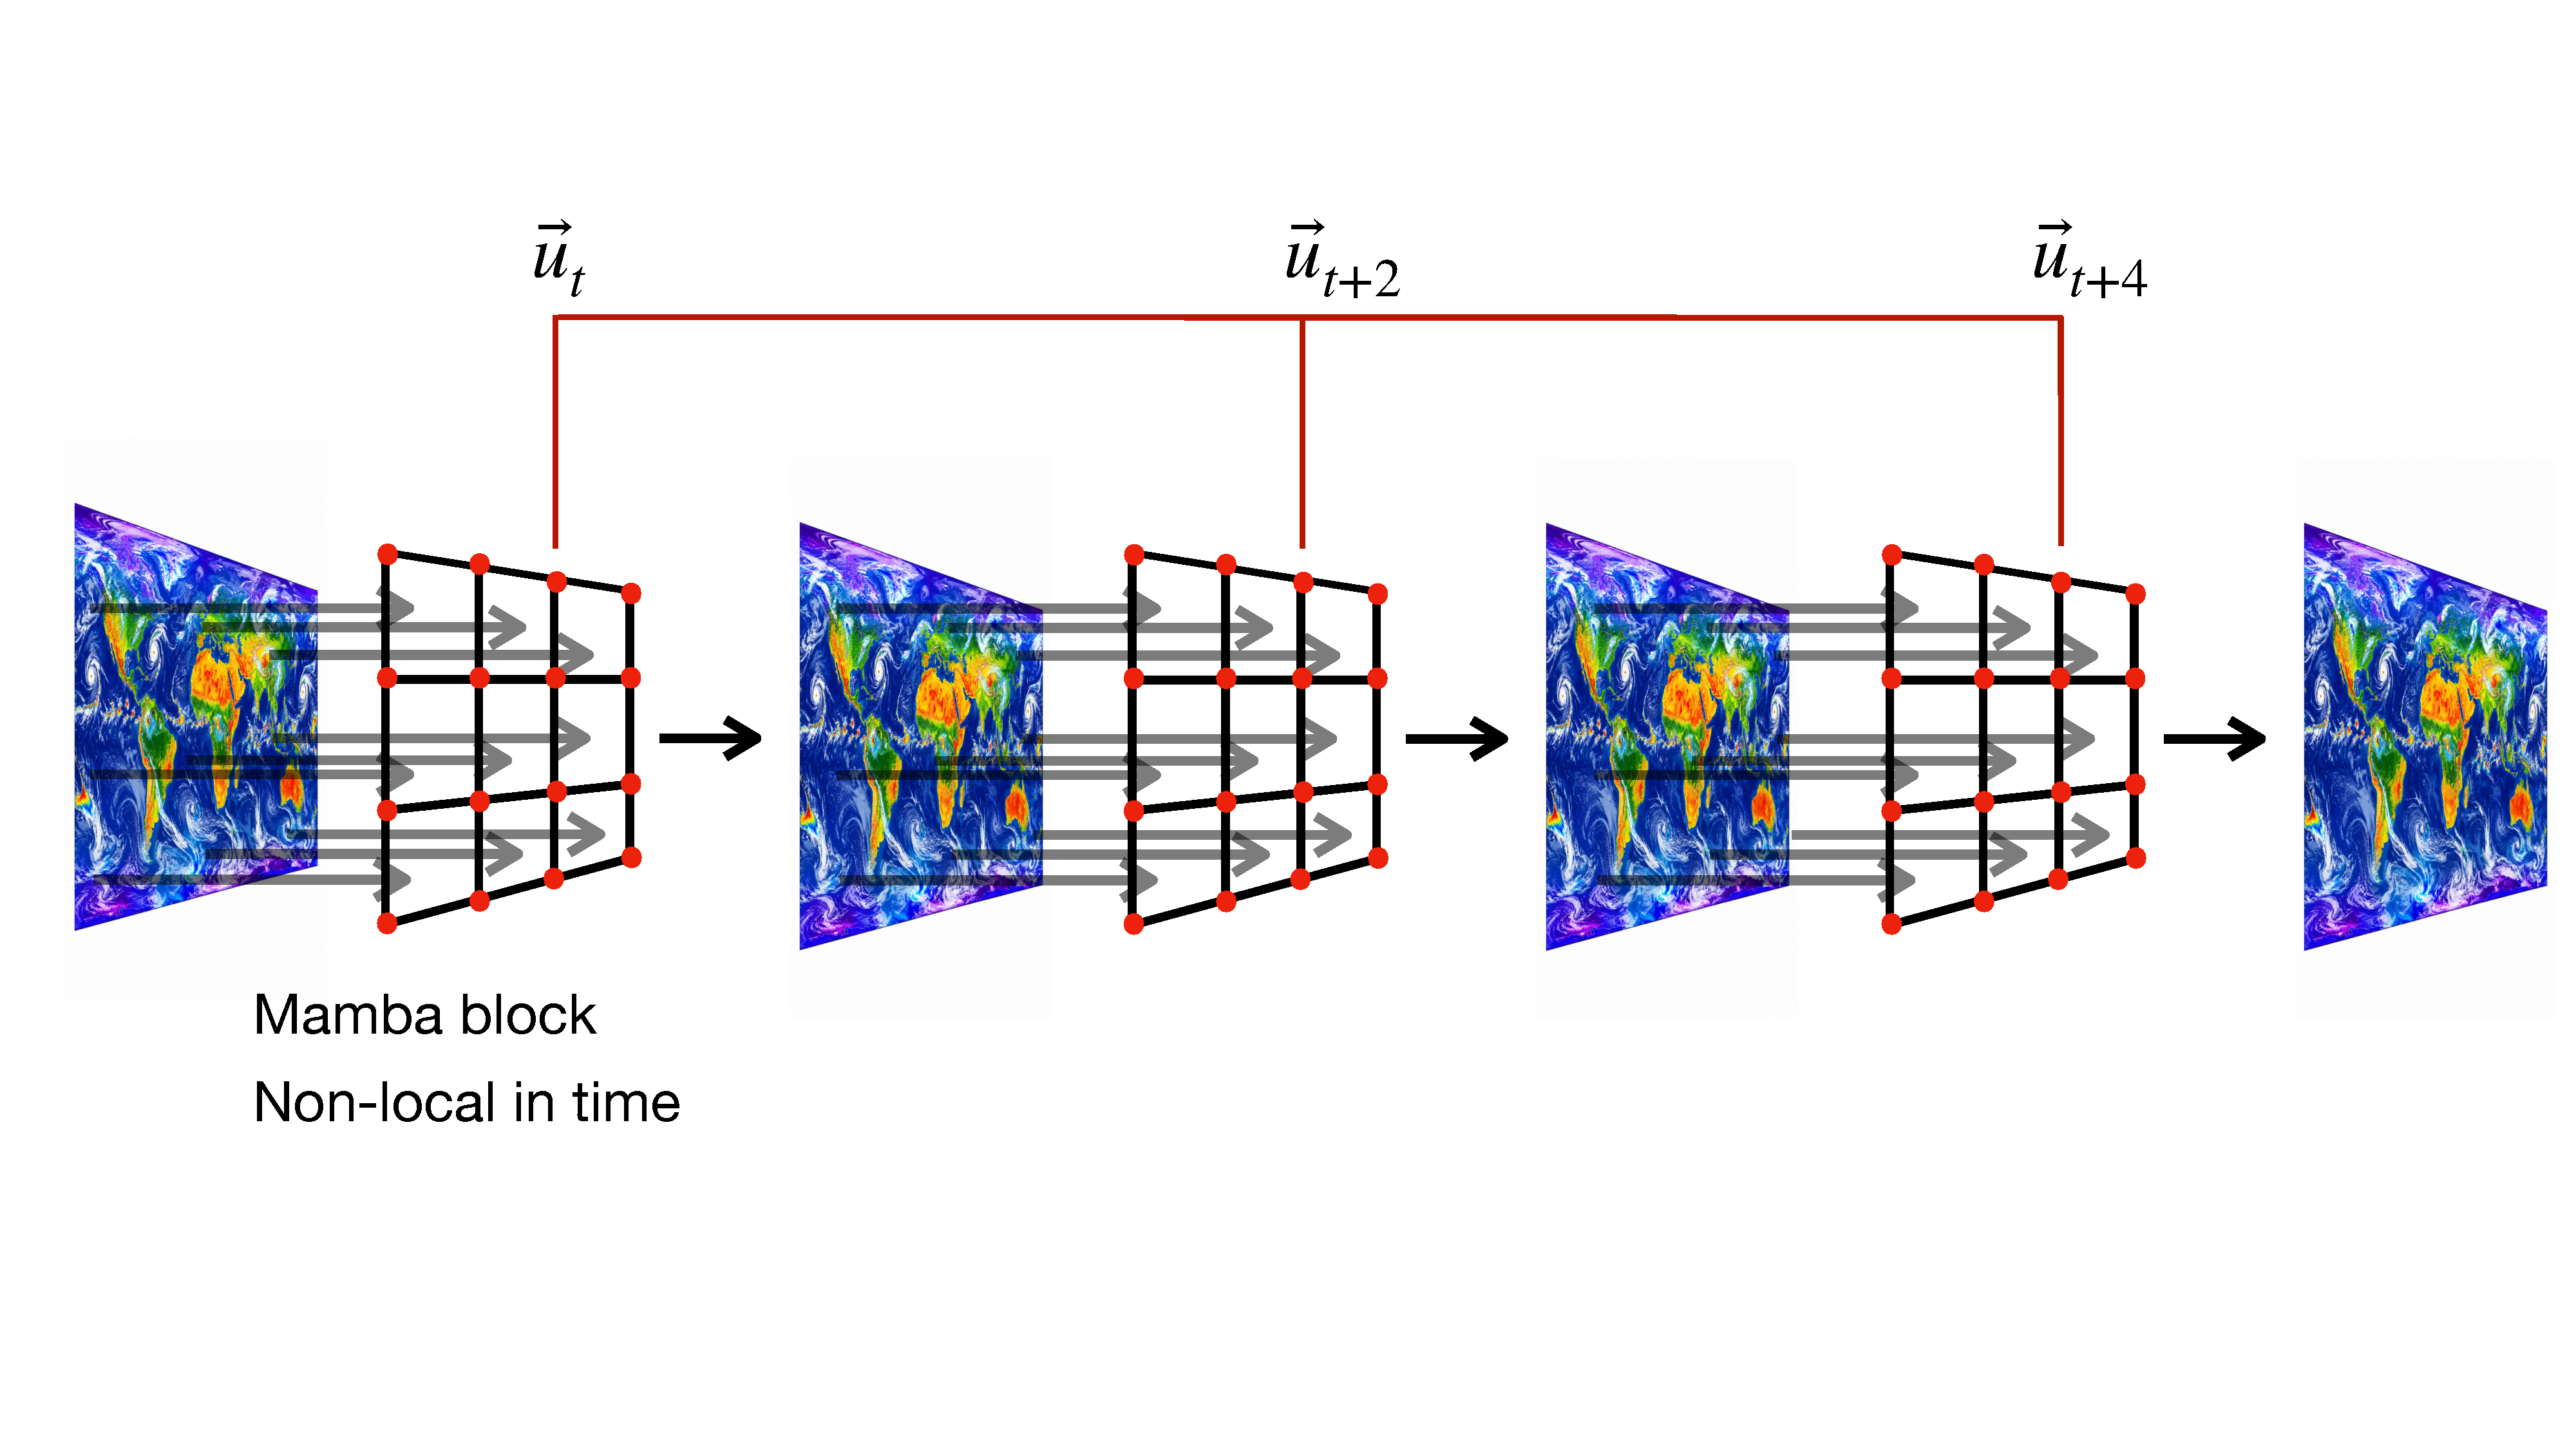
\includegraphics[width=\linewidth,trim=40bp 235bp 5bp 155bp,clip]{Pics/GC_mamba.pdf}
        \caption{Mamba augments mesh processing with persistent temporal states.}
    \end{subfigure}
    \caption{Spatial and temporal processing components. In the experiments, a frozen GraphCast baseline is combined at the output with a separate trainable correction branch containing graph message passing and Mamba.}
    \label{fig:GC_Mamba}
\end{figure}

\subsection{A hybrid GraphCast--Mamba architecture}
We study whether a persistent latent memory improves forecasts beyond the finite input history supplied to a pretrained GraphCast model. GraphCast uses two successive atmospheric states as input; its forecast is Markovian with respect to this augmented state. Our correction branch retains additional temporal information through Mamba states carried across autoregressive steps. This introduces history dependence relative to the baseline input representation. Figure~\ref{fig:GC_Mamba} illustrates the graph and temporal processing components.

\paragraph{GraphCast}
The baseline is a pretrained GraphCast checkpoint. This graph neural network operates on a latitude--longitude grid and an auxiliary mesh, with graph $\mathcal{G}(\mathcal{V}^{\textrm{G}},\mathcal{V}^{\textrm{M}},\mathcal{E}^{\textrm{G2M}},\mathcal{E}^{\textrm{M}},\mathcal{E}^{\textrm{M2G}})$. The vertices $\mathcal{V}^{\textrm{G}}$ represent the meteorological grid and $\mathcal{V}^{\textrm{M}}$ the mesh. Encoding uses grid-to-mesh edges $\mathcal{E}^{\textrm{G2M}}$, followed by $N=16$ mesh message-passing steps over $\mathcal{E}^{\textrm{M}}$ and decoding over mesh-to-grid edges $\mathcal{E}^{\textrm{M2G}}$. Latent node features have width $W_{\textrm{GC}}=512$. The mesh provides a more compact representation for spatial processing than the meteorological grid.

\paragraph{Mamba}
Mamba is an attention-free sequence model based on selective state-space models (SSMs), designed to model long temporal dependencies with computation that scales linearly with sequence length \cite{gu2023Mamba}. A conventional continuous-time SSM maps an input sequence $x(t)$ to a latent memory state $h(t)$ according to
\begin{equation}
    \frac{d h(t)}{dt} = A h(t) + B x(t),
    \qquad
    y(t) = C h(t) + D x(t).
\end{equation}
Here, $A$ is a diagonal matrix that determines how quickly memory decays or evolves, $B$ and $C$ determines how new inputs are written into the state and readout from the state respectively, and $D$ provides a direct input-to-output skip connection. For a single SSM channel, each of the matrices have fixed dimension $d_{\textrm{state}}=16$ and $\Delta$ - is a scalar. If $A$, $B$, and $C$ are fixed, the same linear dynamical system is applied at every time step. For a discrete step size $\Delta$, its exact discretization is
\begin{equation}
    h_t = \bar{A} h_{t-1} + \bar{B}x_t,
    \qquad
    \bar{A} = \exp(\Delta A),
    \qquad
    \bar{B} = A^{-1}\left[\exp(\Delta A)-I\right]B.
\end{equation}

Mamba makes this SSM \emph{selective}: rather than using fixed input and readout matrices and a fixed step size, it computes $B_t$, $C_t$, and $\Delta_t$ from the current input. Thus, the model can decide which information to retain, overwrite, or expose at each time step.

In our model, Mamba operates independently on the temporal sequence of each GraphCast mesh node. Let $x_t^{\mathrm{in}}\in\mathbb{R}^{W_{\textrm{GC}}}$ denote the mesh latent feature at a given node and forecast step. A layer-normalized input is projected into two $d_{\textrm{inner}}$-dimensional branches,
\begin{equation}
    [\tilde{x}_t,z_t]
    =
    W_{\mathrm{in}}\operatorname{LN}(x_t^{\mathrm{in}}),
    \qquad
    \tilde{x}_t,z_t\in\mathbb{R}^{d_{\textrm{inner}}}.
\end{equation}
The first branch, $\tilde{x}_t$, supplies the SSM input. The second branch, $z_t$, is a learned output gate: it does not update the memory state directly, but controls how much of the SSM output is passed onward.

Before entering the SSM, $\tilde{x}_t$ is processed by a depthwise causal one-dimensional convolution with kernel width four:
\begin{equation}
    u_{t,d}
    =
    \operatorname{SiLU}
    \left(
        b^{\mathrm{conv}}_d
        +
        \sum_{k=0}^{d_{\textrm{conv}}-1}
        w^{\mathrm{conv}}_{d,k}\tilde{x}_{t-k,d}
    \right),
    \qquad d=1,\ldots, d_{\textrm{inner}},
\end{equation}
where $\operatorname{SiLU}(a)=a/(1+e^{-a})$. ``Depthwise'' means that each of the $d_{inner}$ channels has its own $d_{\textrm{conv}}$ learned convolution weights $w^{\mathrm{conv}}_{d,k}$ and does not mix with other channels at this stage. ``Causal'' means that $u_t$ depends only on the current input and the three previous inputs, never on future inputs. During autoregressive inference, the preceding three projected inputs are retained in a convolution cache, so this local temporal context continues across forecast calls.

The selective parameters are generated from $u_t$ by learned linear projections:
\begin{equation}
    [r_t,B_t,C_t] = W_xu_t,
    \qquad
    r_t\in\mathbb{R}^{d_t},
    \quad
    B_t,C_t\in\mathbb{R}^{d_{\textrm{state}}},
\end{equation}
\begin{equation}
    \Delta_t
    =
    \operatorname{softplus}(W_\Delta r_t+b_\Delta)
    \in\mathbb{R}^{d_{\textrm{inner}}}.
\end{equation}
Here $d_t=32$ and $d_{\mathrm{state}}=16$. The projection matrices, convolution kernels, and biases are trainable parameters optimized using the forecasting loss. In contrast, $B_t$, $C_t$, and $\Delta_t$ are input-dependent values generated anew at each time step from $u_t$. The softplus function ensures $\Delta_t>0$.

The continuous-time state matrix is diagonal and parameterized as
\begin{equation}
    A_{d,n}=-\exp(A_{\log,d,n}),
    \qquad
    d=1,\ldots,d_{\textrm{inner}},\quad n=1,\ldots,d_{\textrm{state}}.
\end{equation}
Because every element of $A$ is negative, the corresponding factor $\exp(\Delta_{t,d}A_{d,n})$ lies between zero and one, giving stable, decaying memory. The implementation uses the following selective recurrence:
\begin{equation}
    h_{t,d,n}
    =
    \exp\!\left(\Delta_{t,d}A_{d,n}\right)h_{t-1,d,n}
    +
    \Delta_{t,d}B_{t,n}u_{t,d}.
\end{equation}
The first term retains a scaled portion of the previous state, while the second writes the current input into memory. A small $\Delta_{t,d}$ gives slow decay and long memory; a large $\Delta_{t,d}$ gives faster decay and a stronger update from the current input.

The state is read out using the selective vector $C_t$ and a learned skip parameter $D$:
\begin{equation}
    s_{t,d}
    =
    \sum_{n=1}^{16} C_{t,n}h_{t,d,n}
    +
    D_d u_{t,d}.
\end{equation}
Finally, the gate branch $z_t$ modulates this readout, and the result is projected back to the $W_{\textrm{GC}}$-dimensional GraphCast latent space:
\begin{equation}
    o_t
    =
    W_{\mathrm{out}}
    \left[
        s_t\odot\operatorname{SiLU}(z_t)
    \right],
    \qquad
    x_t^{\mathrm{out}}=x_t^{\mathrm{in}}+o_t.
\end{equation}

The principal experiments use $d_{\mathrm{inner}}=16$, an SSM state dimension of $16$ per channel, a causal convolution width of $4$, and a rank-$32$ projection for $\Delta_t$; we also examine $d_{\mathrm{inner}}=32$ and $64$. The SSM state $h_t$ and the three-token convolution cache persist separately for each batch element, mesh node, and Mamba layer across autoregressive forecast steps. The equations above describe one shared group of input-dependent $B_t,C_t$ coefficients. The grouped variant partitions the inner channels into groups with separate $B_t,C_t$ coefficients; the memory ablation compares one and four such groups.



\paragraph{An additive correction with internal temporal memory.}
Let $X_t$ denote the two-frame meteorological input and the associated forcings. The forecast combines the frozen baseline $G_\theta$ with a trainable correction $R_\phi$:
\begin{equation}
    (c_t,h_t)=R_\phi(X_t,h_{t-1}),
    \qquad
    \hat{Y}_t=G_\theta(X_t)+c_t,
    \qquad \theta\ \text{fixed}.
    \label{eq:additive_correction}
\end{equation}
The correction branch has its own grid-to-mesh encoder, mesh processor, and mesh-to-grid decoder. It receives the same meteorological inputs as the baseline, rather than the baseline's latent features. Its mesh processor uses two message-passing steps, each followed by a two-layer Mamba module. Schematically,
\begin{align}
    L_t^{(0)} &= \operatorname{Encode}_\phi(X_t),\\
    \widetilde{L}_t^{(k)} &= \operatorname{GNN}^{(k)}_\phi(L_t^{(k-1)}),\\
    (L_t^{(k)},h_t^{(k)})
    &=\operatorname{TemporalModule}^{(k)}_\phi
       (\widetilde{L}_t^{(k)},h_{t-1}^{(k)}),\qquad k=1,2,\\
    c_t &= \operatorname{Decode}_\phi(L_t^{(2)}).
\end{align}
Each temporal module contains the residual Mamba updates described above; the state notation includes both SSM states and convolution caches. The output correction is initialized to zero. This formulation is additive at the forecast output and uses temporal processing within the residual GNN branch. During autoregressive forecasting, the combined prediction is fed into the next input, and the temporal states carry information from the preceding trajectory.

\section{Numerical results}
\label{sec:numerical}
We focus on $1^\circ$ GraphCast-small models and ask two questions: does a learned correction improve long-range forecast skill, and does persistent temporal memory contribute beyond the additional trainable capacity? We first report forecast skill, then isolate the effect of state carry, and finally examine sensitivity to training choices.

\subsection{Evaluation protocol and forecast loss}
The matched-start evaluations use 32 forecast initializations from 2022 and 40 six-hour forecast steps, corresponding to ten days. Forecasts start with zero temporal state and use the full combined prediction as feedback, without a history warm start. The pretrained GraphCast baseline remains frozen during correction training. The principal correction branch has spatial width $512$, two message-passing steps, and Mamba inner dimension $16$.

Our primary metric is the original GraphCast normalized weighted mean-squared error, including its difference-standard-deviation normalization, latitude weights, pressure-level weights, and variable weights. If $\ell_{i,k}^{\mathrm{model}}$ and $\ell_{i,k}^{\mathrm{GC}}$ are the losses for start $i$ and lead $k$, the rollout loss reduction is
\begin{equation}
    \mathcal{I}_{1:40}
    =100\left(1-
      \frac{\sum_{i=1}^{32}\sum_{k=1}^{40}\ell_{i,k}^{\mathrm{model}}}
           {\sum_{i=1}^{32}\sum_{k=1}^{40}\ell_{i,k}^{\mathrm{GC}}}
    \right).
    \label{eq:rollout_reduction}
\end{equation}
Day-ten reduction uses only $k=40$. We aggregate losses before taking the ratio; these percentages are neither RMSE reductions nor arithmetic averages of per-lead percentages. Each evaluated model uses its saved matched baseline. The older reset study reconstructs an approximate loss from channel RMSEs and is explicitly identified as such below.

\clearpage
\begin{figure}[!t]
    \centering
    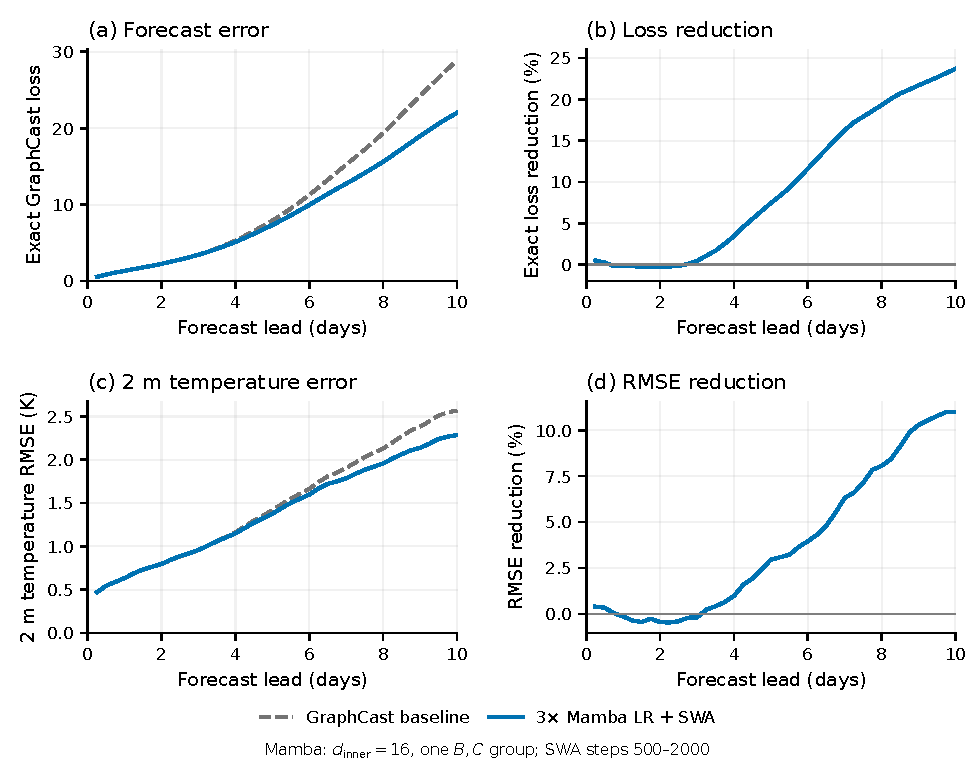
\includegraphics[width=\linewidth]{Graphs/main_v2/exact_gc_loss.pdf}
    \caption{Forecast skill of the $d_{\mathrm{inner}}=16$ correction trained with a threefold Mamba learning rate and stochastic weight averaging (SWA) at $1^\circ$ on 32 matched starts. Top: exact GraphCast loss and per-lead loss reduction. Bottom: cosine-latitude-weighted $2$\,m temperature RMSE (K) and RMSE reduction on the same starts. Reductions are relative to its paired GraphCast baseline. Training and model-selection details are given in Appendix~\ref{app:training}.}
    \label{fig:res1_forecast}
\end{figure}

\subsection{Improved skill at longer forecast leads}
Figure~\ref{fig:res1_forecast} shows the $d_{\mathrm{inner}}=16$ correction trained with a $3\times$ Mamba learning rate and SWA. It reduces exact aggregate ten-day loss by $16.34\%$ and day-ten loss by $23.68\%$. The per-lead reduction grows from $3.45\%$ at day four to $16.25\%$ at day seven and $23.68\%$ at day ten. Day-one loss reduction is $-0.13\%$, indicating a small degradation; short-lead skill is largely preserved rather than uniformly improved. At day ten, $2$\,m temperature RMSE is $2.29$\,K, a $10.98\%$ reduction relative to the paired baseline.

\clearpage
\begin{figure}[!t]
    \centering
    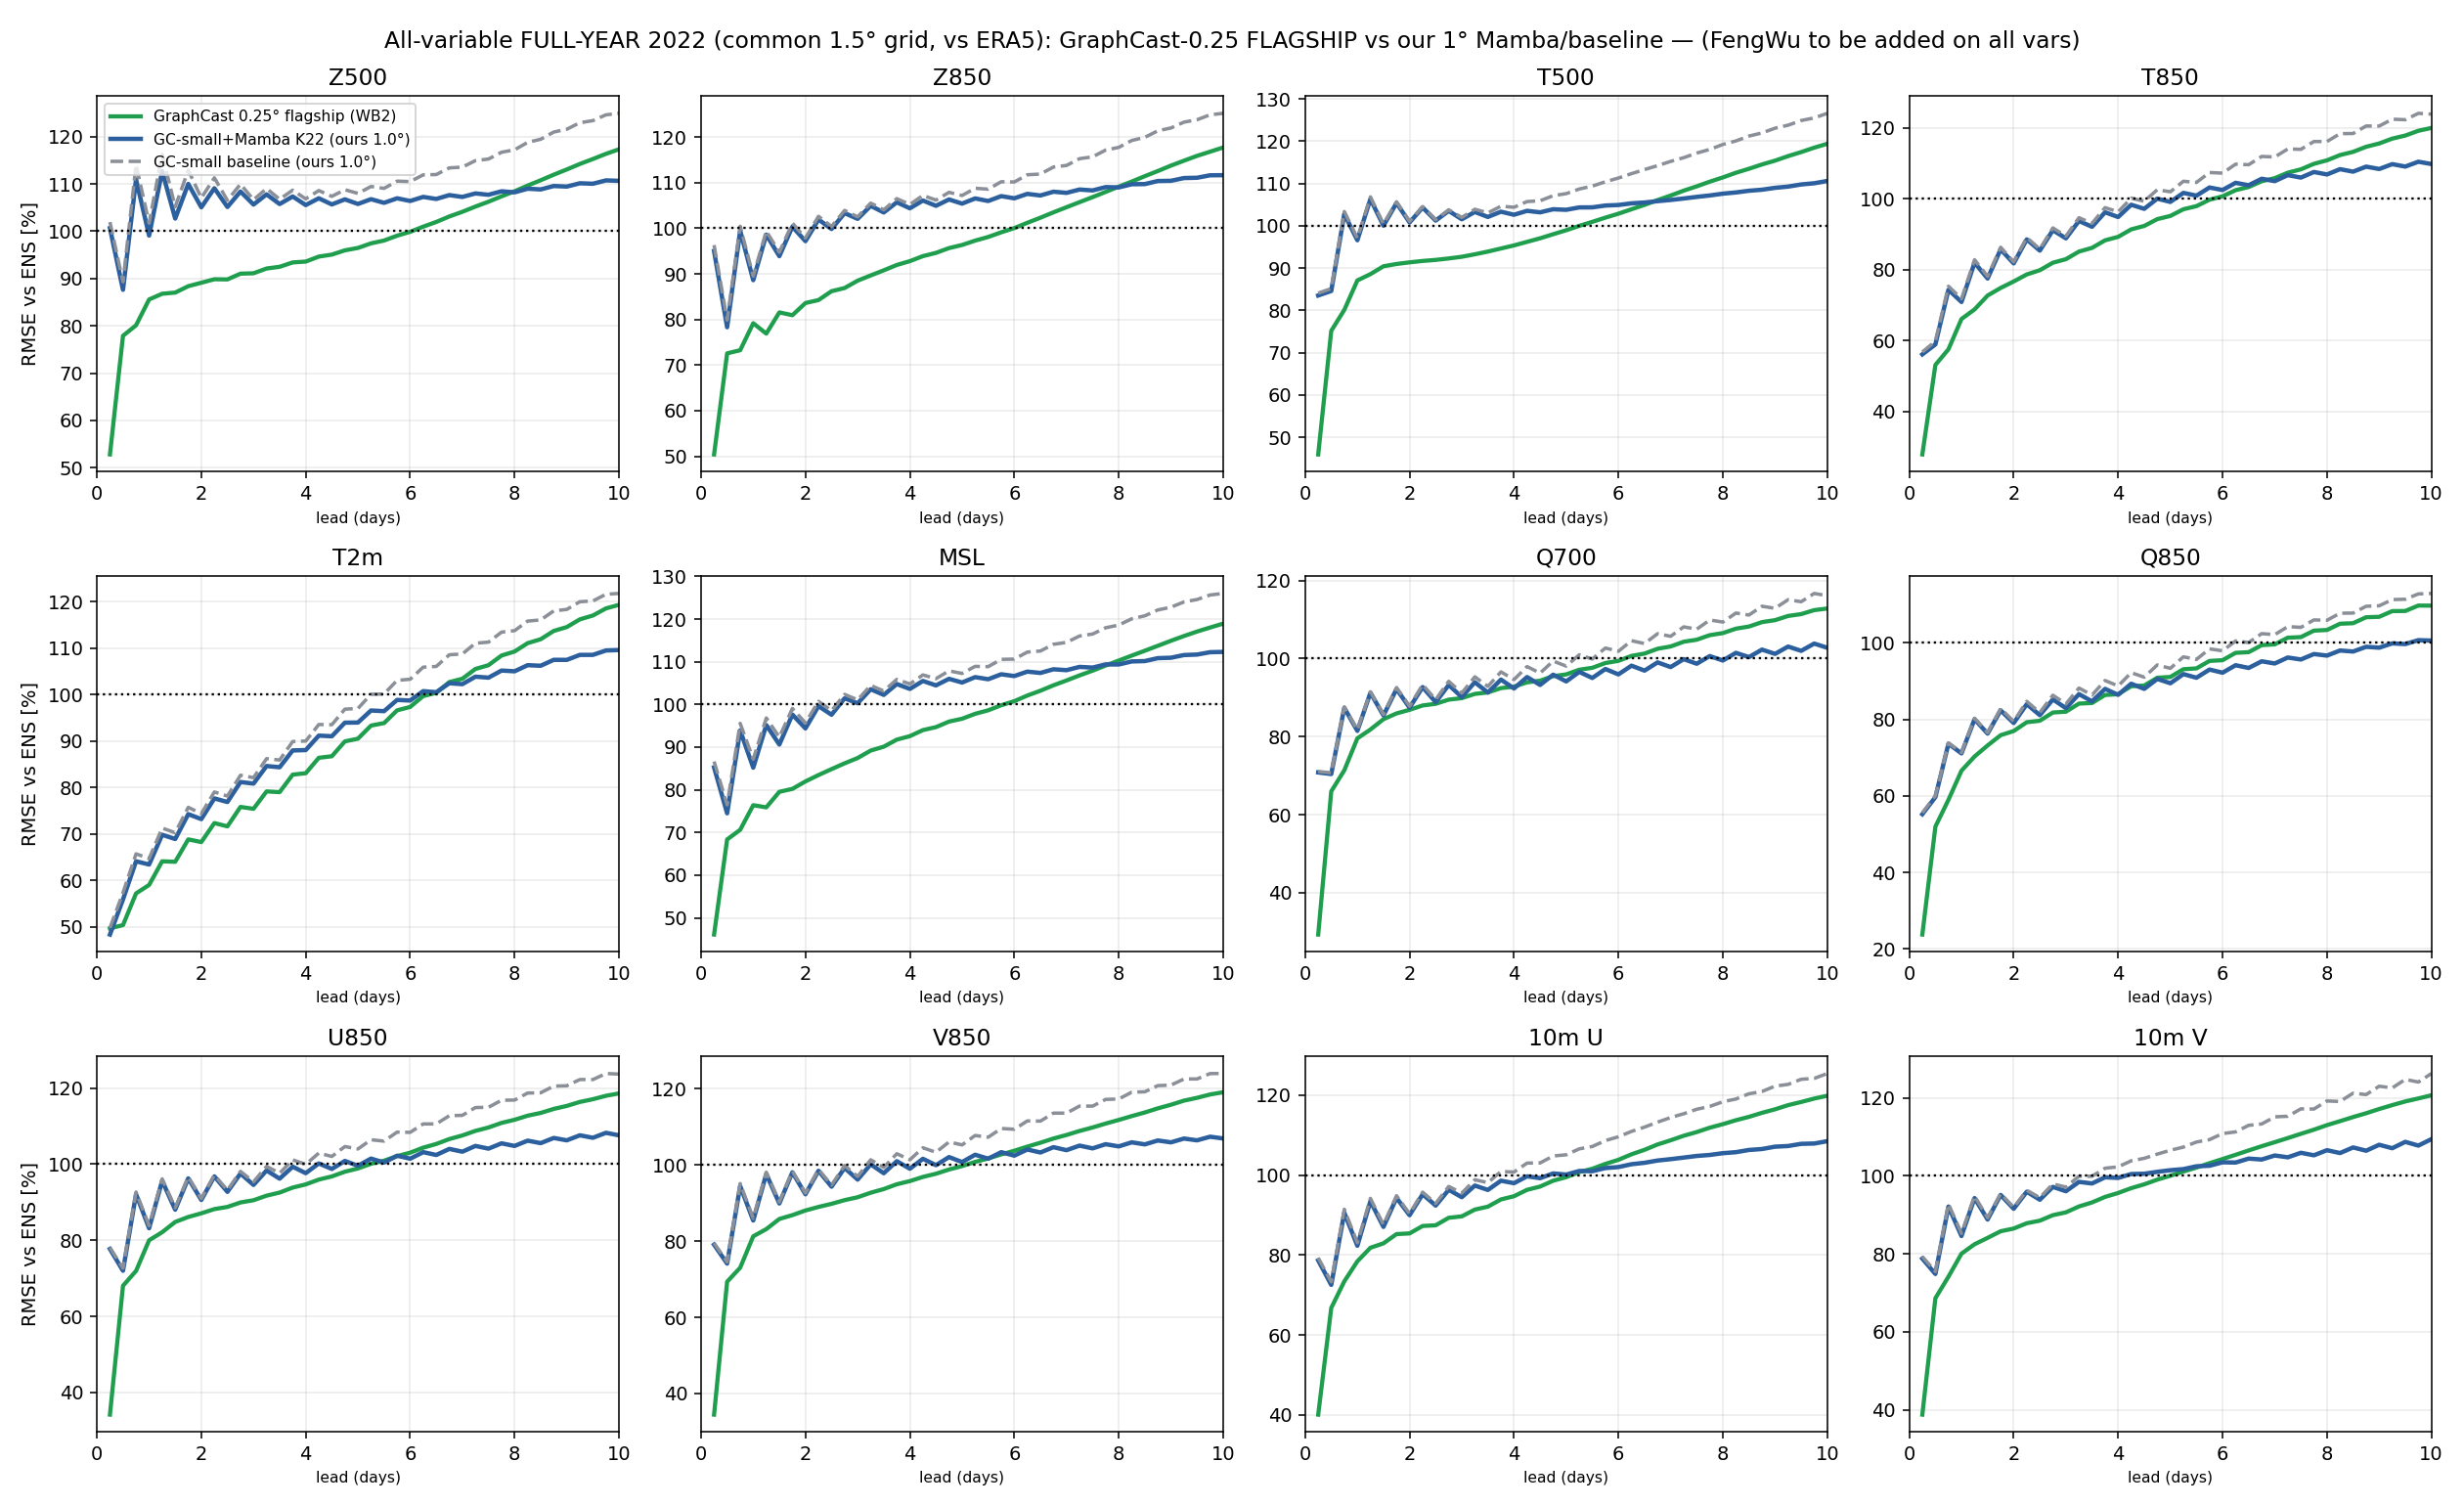
\includegraphics[width=\linewidth]{Graphs/add_mamba.png}
    \caption{Complete common-grid comparison. The quantities span geopotential, temperature, sea-level pressure, humidity, and wind. Blue is the archived K22 correction, dashed gray its GraphCast-small baseline, and green the $0.25^\circ$ reference. Forecasts are verified on a common $1.5^\circ$ grid, with RMSE normalized to the displayed ENS reference ($100\%$ denotes equal RMSE). This historical comparison is separate from the matched-start evaluations in Figure~\ref{fig:res1_forecast}.}
    \label{fig:res1_all_variables}
\end{figure}

We further assess forecast skill for the meteorological quantities in Figure~\ref{fig:res1_all_variables}, considered in the original GraphCast study~\cite{lam2023graphcast}. These panels compare forecasts on a common $1.5^\circ$ verification grid and again show more favorable error growth with forecast lead time for our corrected $1^\circ$ model than for its uncorrected baseline. Note that the model output resolution and verification resolution are different quantities. Remarkably, in this comparison, the corrected $1^\circ$ model achieves lower errors at longer leads even than the $0.25^\circ$ GraphCast-large reference, despite its coarser spatial resolution and the substantial computational investment in training the reference model: approximately four weeks on 32 TPU v4 devices~\cite{lam2023graphcast}.

\clearpage
\begin{figure}[!t]
    \centering
    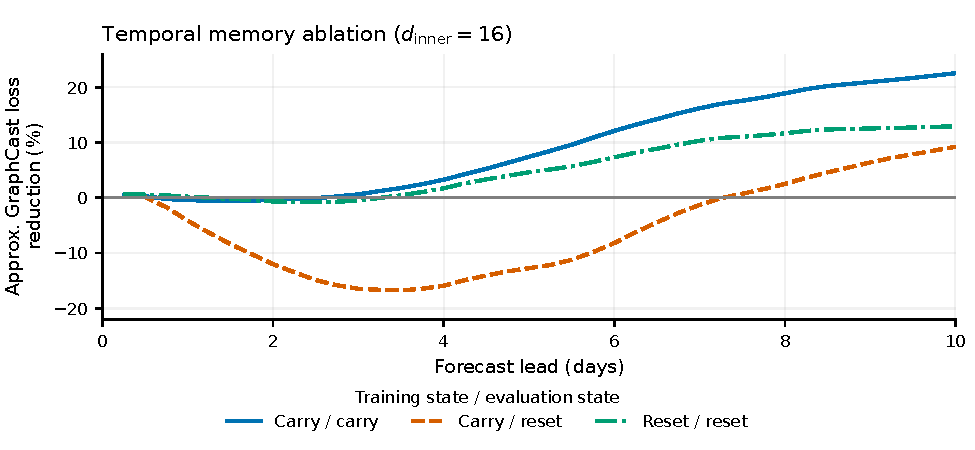
\includegraphics[width=\linewidth]{Graphs/main_v2/memory_reset.pdf}
    \caption{Persistent memory improves long-lead forecasts. All three policies use the same architecture with $d_{\mathrm{inner}}=16$, one $B,C$ group, and SWA over updates 2k--8k. Carry/carry retains state during training and forecasting; carry/reset clears state during forecasting; reset/reset clears it during both. Carry/carry achieves the largest day-ten loss reduction. Results use 32 matched cold starts and 40 six-hour leads; positive values indicate lower loss than the paired GraphCast baseline. Loss is reconstructed approximately from saved channel RMSEs.}
    \label{fig:memory_reset}
\end{figure}

\subsection{Evidence for useful temporal memory}
\label{sec:memory_ablation}
A correction branch can improve forecasts through additional spatial capacity as well as temporal memory. To distinguish these contributions, we compare three policies: state carry during both training and evaluation; state carry during training followed by resetting at every evaluation step; and a separately trained model with resetting at every training and evaluation step. Resetting zeros both the SSM state and the convolution cache. The carry-trained and reset-trained runs have the same architecture, data settings, optimizer, and training seed; their temporal-state policy differs.

Figure~\ref{fig:memory_reset} isolates the temporal-state policy for a fixed $d_{\mathrm{inner}}=16$ model. Carry/carry gives the strongest long-lead improvement: day-ten approximate loss reduction is $22.52\%$, compared with $9.24\%$ for carry/reset and $12.91\%$ for reset/reset. Retaining memory therefore adds $13.28$ percentage points relative to resetting the trained state at inference and $9.62$ percentage points relative to training and evaluating without persistent state. Additional group settings and averaging windows are reported in Appendix~\ref{app:memory_windows}.

The inference-time reset demonstrates dependence on the learned state, but also introduces a train--evaluation mismatch. The separately trained reset control is therefore essential: it retains the trainable correction architecture while removing persistent temporal context. Its smaller long-lead benefit supports a contribution from memory beyond additional correction capacity. This is evidence for useful history dependence relative to the baseline's two-frame input representation. The experiment does not identify a unique physical memory kernel or isolate the SSM contribution from that of the convolution cache.

\clearpage
\subsection{Sensitivity to inner dimension and temporal learning rate}
\label{sec:training_sensitivity}
Table~\ref{tab:res1_skill} compares inner dimensions 16 and 32 under two training methods: joint learning rates, which use equal learning rates for the spatial and Mamba parameters of the correction branch, and a $3\times$ Mamba learning rate with the spatial learning rate unchanged. All four configurations use the same training schedule and SWA window. Under joint learning rates, the dimension-32 correction achieves larger aggregate and day-ten loss reductions than the dimension-16 correction. With a $3\times$ Mamba learning rate, the ordering reverses: the dimension-16 correction shown in Figure~\ref{fig:res1_forecast} achieves the largest reductions in the table. The benefit of increasing inner dimension therefore depends on the temporal learning rate in these runs. Each run starts from its own trained warm-up parameters, so these are comparisons of complete training runs. Appendix~\ref{app:training} gives the training details and the additional $0.3\times$ Mamba learning-rate results.

\begin{table}[!h]
    \centering
    \caption{Inner dimension and Mamba learning-rate comparison at $1^\circ$ on the matched 32-start development evaluation. Entries are exact GraphCast loss reductions (\%); bold marks the largest value in each metric column. All runs use spatial width 512, one $B,C$ group, batch size four, the same training schedule, and SWA over branch updates 500, 1,000, 1,500, and 2,000. The spatial learning rate is unchanged; $1\times$ denotes joint learning rates.}
    \label{tab:res1_skill}
    \small
    \begin{tabular}{rlrr}
        \toprule
        $d_{\mathrm{inner}}$ & Mamba LR multiplier & Ten-day aggregate & Day ten \\
        \midrule
        16 & $1\times$ (joint) & 15.67 & 22.44 \\
        32 & $1\times$ (joint) & 16.29 & 23.32 \\
        \addlinespace
        16 & $3\times$ & \textbf{16.34} & \textbf{23.68} \\
        32 & $3\times$ & 15.73 & 22.75 \\
        \bottomrule
    \end{tabular}
\end{table}

\paragraph{Scope of the evidence.}
The exact-loss studies use one training seed and a 32-start development set used in model selection. We therefore report descriptive improvements without significance claims. The memory controls support the contribution of persistent state in the tested configuration; they do not directly establish the same attribution for every model. Evaluation on forecast dates reserved from selection, with matched uncertainty estimates and exact-loss reset controls, would strengthen the quantitative conclusions.

% Keep all main-text floats ahead of the references and appendices.
\FloatBarrier
\bibliographystyle{plainnat}
\bibliography{bib}

\clearpage
\appendix
\begin{figure}[!t]
    \centering
    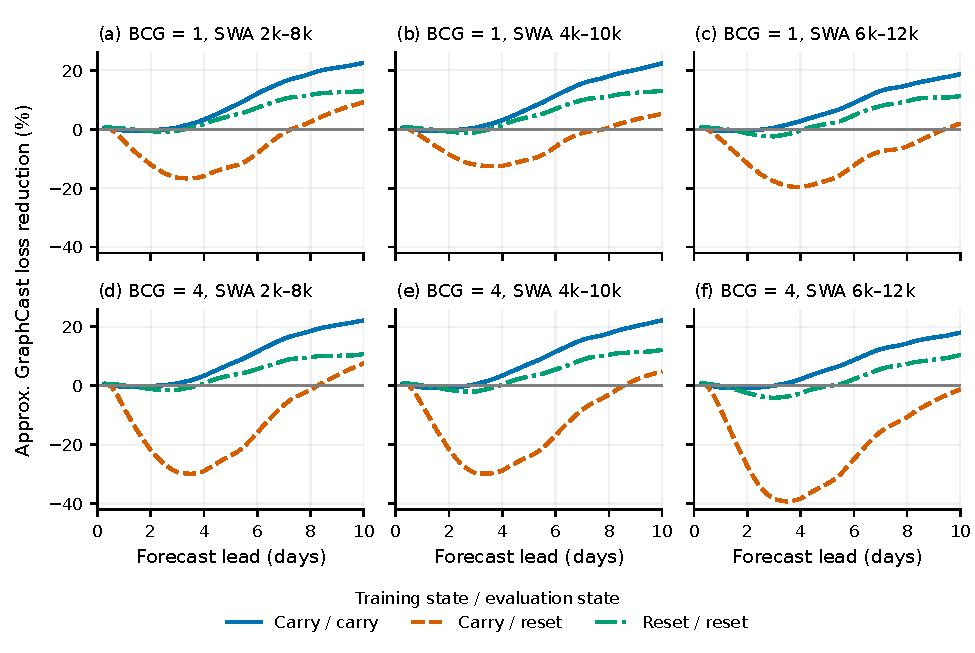
\includegraphics[width=\linewidth]{Graphs/main_v2/memory_reset_all.pdf}
    \caption{Complete temporal-state comparison. Column titles specify the SWA windows, and rows specify one or four $B,C$ groups. All panels use approximate GraphCast loss reconstructed from saved channel RMSEs.}
    \label{fig:memory_all_windows}
\end{figure}

\section{Memory ablation across averaging windows}
\label{app:memory_windows}
The full reset study fixes $d_{\mathrm{inner}}=16$ and varies the number of $B,C$ groups (one or four) and the SWA window (2k--8k, 4k--10k, or 6k--12k updates). Carry/carry achieves the largest day-ten reduction in each panel of Figure~\ref{fig:memory_all_windows}. The SWA windows overlap and are derived from the same training trajectories; they are sensitivity checks, not independent seed repetitions. The approximate metric and the distinct train/evaluation reset policies are the same as in Section~\ref{sec:memory_ablation}. Each curve uses its saved baseline (maximum baseline channel-RMSE difference across the full study: $0.56\%$); exact pole weighting cannot be recovered from these channel summaries.

\section{Training choices and checkpoint averaging}
\label{app:training}
\paragraph{Training methods and model selection.}
Table~\ref{tab:res1_skill} reports four SWA configurations from the temporal learning-rate study: joint learning rates and a $3\times$ Mamba learning rate, each with inner dimensions 16 and 32. Joint learning rates apply the same rate to the spatial and Mamba parameters of the correction branch; the $3\times$ configuration increases only the Mamba rate. The pretrained GraphCast parameters remain frozen in all cases. Figure~\ref{fig:res1_forecast} uses the dimension-16, $3\times$ Mamba-LR SWA configuration, which has the largest aggregate and day-ten exact-loss reductions among the completed SWA configurations in the reported optimizer and learning-rate studies. This selection uses the matched 32-start development evaluation and does not establish optimality on an independent test set.

\paragraph{Optimizer study.}
The optimizer study varies peak learning rate ($10^{-4}$ or $5\times10^{-5}$), Adam moments, temporal initialization scheme (legacy or Mamba1), and the paired inner-dimension/group settings (16/1 or 64/4). The latter changes two factors simultaneously and does not isolate inner dimension. Runs use 10,000 updates, seed 22, a 200-update warm-up, cosine decay to one tenth of the peak learning rate, and weight decay $10^{-4}$. The correction is trained with closed-loop feedback, 24-step backpropagation windows, a 20-step autoregressive tail, and loss across all 24 steps. The correction contribution to the feedback is stop-gradient, while temporal-state gradients propagate within the backpropagation window.

Each run screens periodic checkpoints and three SWA windows on eight forecast starts. The selected checkpoint and SWA are then evaluated on the matched 32 starts. Selection uses these development evaluations, so the study does not represent an untouched test-set comparison.

Day-ten reductions for the 22 completed selected SWA configurations range from $13.47\%$ to $23.21\%$. The configuration at the upper end uses Mamba1 initialization, inner dimension 16, one $B,C$ group, learning rate $10^{-4}$, and AdamW moments $(0.9,0.98)$; its aggregate loss reduction is $16.28\%$.

\paragraph{Temporal learning rate and inner dimension.}
The temporal learning-rate study keeps spatial width 512 and one $B,C$ group while varying inner dimension and the Mamba learning-rate multiplier. Each arm uses its own 500-update warm-up followed by 2,000 branch updates at batch size four. The base peak learning rate is $10^{-4}$ with AdamW moments $(0.9,0.98)$. Table~\ref{tab:lr_sensitivity} extends the four configurations in Table~\ref{tab:res1_skill} with the $0.3\times$ Mamba learning rate at each inner dimension. All six use SWA over branch updates 500, 1,000, 1,500, and 2,000. The warm-up parameter values differ across arms despite the common training seed, so the comparisons describe complete training runs rather than isolated learning-rate interventions.

Under joint learning rates, the dimension-32 SWA correction exceeds the dimension-16 correction's aggregate loss reduction by $0.62$ percentage points. Under the $3\times$ Mamba learning rate, the dimension-32 correction instead has a smaller aggregate reduction by $0.61$ percentage points. The $0.3\times$ Mamba-LR SWA results also favor dimension 32, while each dimension attains its largest reductions at a different multiplier: $3\times$ for dimension 16 and $1\times$ for dimension 32. These observations do not establish a monotonic benefit from increasing inner dimension or temporal learning rate.

\begin{table}[htbp]
    \centering
    \caption{Exact GraphCast loss reduction (\%) for the learning-rate study's SWA models. Spatial learning rate is unchanged across these six arms; the multiplier applies to Mamba parameters. All evaluations contain the same 32 starts.}
    \label{tab:lr_sensitivity}
    \small
    \begin{tabular}{rrrr}
        \toprule
        $d_{\mathrm{inner}}$ & Mamba LR multiplier & Ten-day aggregate & Day ten \\
        \midrule
        16 & $0.3\times$ & 14.70 & 21.98 \\
        16 & $1\times$   & 15.67 & 22.44 \\
        16 & $3\times$   & \textbf{16.34} & \textbf{23.68} \\
        32 & $0.3\times$ & 15.82 & 22.96 \\
        32 & $1\times$   & 16.29 & 23.32 \\
        32 & $3\times$   & 15.73 & 22.75 \\
        \bottomrule
    \end{tabular}
\end{table}

\begin{samepage}
\paragraph{Stochastic weight averaging.}
SWA averages model parameter values from saved checkpoints to reduce dependence on a single training iterate \cite{izmailov2019averagingweightsleadswider}. Every configuration in Tables~\ref{tab:res1_skill} and~\ref{tab:lr_sensitivity} averages four checkpoints at branch updates 500, 1,000, 1,500, and 2,000. The dimension-16 Mamba1-initialized optimizer-study configuration described above averages seven checkpoints, saved every 1k updates from 2k through 8k. These are parameter averages, not ensembles of independent forecast predictions. Evaluation starts temporal state from zero, including for SWA models.
\end{samepage}
\end{document}
